%-----------------------------------------------------------------
%	BASIC DOCUMENT LAYOUT
%-----------------------------------------------------------------
\documentclass[paper=a4, fontsize=12pt, twoside=semi]{scrartcl}
\usepackage[T1]{fontenc}
\usepackage[utf8]{inputenc}
\usepackage{lmodern}
\usepackage{microtype}
\usepackage[catalan]{babel}
\usepackage[fixlanguage]{babelbib}
\selectbiblanguage{catalan}

% Sectioning layout
\addtokomafont{sectioning}{\normalfont\scshape}
\usepackage{tocstyle}
\usetocstyle{standard}
\renewcommand*\descriptionlabel[1]{\hspace\labelsep\normalfont\bfseries{#1}}

% Empty pages
\usepackage{etoolbox}
\pretocmd{\section}{\cleardoubleevenemptypage}{}{}
\pretocmd{\part}{\cleardoubleevenemptypage\thispagestyle{empty}}{}{}
\renewcommand\partheadstartvskip{\clearpage\null\vfil}
\renewcommand\partheadmidvskip{\par\nobreak\vskip 20pt\thispagestyle{empty}}

% Paragraph indentation behaviour
\setlength{\parindent}{0pt}
\setlength{\parskip}{0.3\baselineskip plus2pt minus2pt}
\newcommand{\sk}{\medskip\noindent}

% Fancy header and footer
\usepackage{fancyhdr}
\pagestyle{fancyplain}
\fancyhead[LO]{\thepage}
\fancyhead[CO]{}
\fancyhead[RO]{\nouppercase{\mytitle}}
\fancyhead[LE]{\nouppercase{\leftmark}}
\fancyhead[CE]{}
\fancyhead[RE]{\thepage}
\fancyfoot{}
\renewcommand{\headrulewidth}{0.3pt}
\renewcommand{\footrulewidth}{0pt}
\setlength{\headheight}{13.6pt}

%-----------------------------------------------------------------
%	MATHS AND SCIENCE
%-----------------------------------------------------------------
\usepackage{amsmath,amsfonts,amsthm,amssymb}
\usepackage{xfrac}
\usepackage[a]{esvect}
\usepackage{chemformula}
\usepackage{graphicx}

% SI units
\usepackage[separate-uncertainty=true]{siunitx}
	%\DeclareSIUnit\micron{\micro\metre}

% Custom commands and operators
\newcommand*{\dif}{\mathrm{d}}
\newcommand*{\diff}{\mathop{}\!\mathrm{d}}
\newcommand*{\der}[3][]{\frac{\dif^{#1}#2}{\dif #3^{#1}}}
\newcommand*{\pder}[3][]{\frac{\partial^{#1}#2}{\partial #3^{#1}}}

\newcommand*{\abs}[1]{\left| #1 \right|}
\newcommand*{\avg}[1]{\left< #1 \right>}
\newcommand*{\norm}[1]{\| #1 \|}
\newcommand*{\eval}[1]{\left. #1 \right|}

\newcommand*{\vnabla}{\vec{\nabla}}
\newcommand*{\grad}[1]{\vnabla #1}
\let\divsymb=\div
\renewcommand*{\div}[1]{\vnabla \cdot #1}
\newcommand*{\rot}[1]{\vnabla \times #1}

% Dirac quantum notation
%\newcommand{\ket}[1]{\left| #1 \right>} % for Dirac kets
%\newcommand{\bra}[1]{\left< #1 \right|} % for Dirac bras
%\newcommand{\braket}[2]{\left< #1 \vphantom{#2} \right| \left. #2 \vphantom{#1} \right>} % for Dirac brackets
%\newcommand{\matrixel}[3]{\left< #1 \vphantom{#2#3} \right| #2 \left| #3 \vphantom{#1#2} \right>} % for Dirac matrix elements

% FLA-style notation for matrices
\usepackage{stackengine}
\newcommand*{\vecsign}{\mathchar"017E}
\newcommand*{\dvecsign}{\smash{\stackon[-2.60pt]{\vecsign}{\rotatebox{180}{$\vecsign$}}}}
\newcommand*{\mat}[1]{\def\useanchorwidth{T}\stackon[-5.4pt]{\mathcal{#1}}{\,\dvecsign}}
\stackMath

% Matrices in (A|B) form via [c|c] option
\makeatletter
\renewcommand*\env@matrix[1][*\c@MaxMatrixCols c]{%
  \hskip -\arraycolsep
  \let\@ifnextchar\new@ifnextchar
  \array{#1}}
\makeatother

%-----------------------------------------------------------------
%	OTHER PACKAGES
%-----------------------------------------------------------------
\usepackage{environ}

% Plots and graphics
\usepackage{pgfplots}
\usepackage{tikz}
\usepackage{color}
	\makeatletter
		\color{black}
		\let\default@color\current@color
	\makeatother

% Richer enumerate, figure, and table support
\usepackage{enumerate}
\usepackage{float}
\usepackage{booktabs}
	%\setlength{\intextsep}{8pt}
\numberwithin{equation}{section}
\numberwithin{figure}{section}
\numberwithin{table}{section}

% No indentation after certain environments
\makeatletter
\newcommand*\NoIndentAfterEnv[1]{%
	\AfterEndEnvironment{#1}{\par\@afterindentfalse\@afterheading}}
\makeatother
%\NoIndentAfterEnv{thm}
\NoIndentAfterEnv{defi}
\NoIndentAfterEnv{example}
\NoIndentAfterEnv{table}

% Misc packages
\usepackage{ccicons}
\usepackage{lipsum}

%-----------------------------------------------------------------
%	THEOREMS
%-----------------------------------------------------------------
\usepackage{thmtools}

% Proofatend environment
\makeatletter
\providecommand{\@fourthoffour}[4]{#4}
\newcommand\fixstatement[2][\proofname\space del]{%
	\ifcsname thmt@original@#2\endcsname
		\AtEndEnvironment{#2}{%
			\xdef\pat@label{\expandafter\expandafter\expandafter
				\@fourthoffour\csname thmt@original@#2\endcsname\space\@currentlabel}%
			\xdef\pat@proofof{\@nameuse{pat@proofof@#2}}%
		}%
	\else
		\AtEndEnvironment{#2}{%
			\xdef\pat@label{\expandafter\expandafter\expandafter
				\@fourthoffour\csname #1\endcsname\space\@currentlabel}%
			\xdef\pat@proofof{\@nameuse{pat@proofof@#2}}%
		}%
	\fi
	\@namedef{pat@proofof@#2}{#1}%
}
\globtoksblk\prooftoks{1000}
\newcounter{proofcount}
\NewEnviron{proofatend}{%
	\edef\next{%
		\noexpand\begin{proof}[\pat@proofof\space\pat@label]%
		\unexpanded\expandafter{\BODY}}%
	\global\toks\numexpr\prooftoks+\value{proofcount}\relax=\expandafter{\next\end{proof}}
	\stepcounter{proofcount}}
\def\printproofs{%
	\count@=\z@
	\loop
		\the\toks\numexpr\prooftoks+\count@\relax
			\ifnum\count@<\value{proofcount}%
			\advance\count@\@ne
	\repeat}
\makeatother

% Theroems layout
\declaretheoremstyle[
    spaceabove=6pt, spacebelow=6pt,
    headfont=\normalfont,
    notefont=\mdseries, notebraces={(}{)},
    bodyfont=\small,
    postheadspace=1em,
]{small}

\declaretheorem[style=plain,name=Teorema,qed=$\square$,numberwithin=section]{thm}
\declaretheorem[style=plain,name=Corol·lari,qed=$\square$,sibling=thm]{cor}
\declaretheorem[style=plain,name=Lemma,qed=$\square$,sibling=thm]{lem}
\declaretheorem[style=definition,name=Definició,qed=$\blacksquare$,numberwithin=section]{defi}
\declaretheorem[style=definition,name=Exemple,qed=$\blacktriangle$,numberwithin=section]{example}
\declaretheorem[style=small,name=Demostració,numbered=no,qed=$\square$]{sproof}
\fixstatement{thm}
\fixstatement[Demostració del]{lem}

%-----------------------------------------------------------------
%	ELA MOTHERFUCKING GEMINADA
%-----------------------------------------------------------------
\def\xgem{%
	\ifmmode
		\csname normal@char\string"\endcsname l%
	\else
		\leftllkern=0pt\rightllkern=0pt\raiselldim=0pt
		\setbox0\hbox{l}\setbox1\hbox{l\/}\setbox2\hbox{.}%
		\advance\raiselldim by \the\fontdimen5\the\font
		\advance\raiselldim by -\ht2
		\leftllkern=-.25\wd0%
		\advance\leftllkern by \wd1
		\advance\leftllkern by -\wd0
		\rightllkern=-.25\wd0%
		\advance\rightllkern by -\wd1
		\advance\rightllkern by \wd0
		\allowhyphens\discretionary{-}{}%
		{\kern\leftllkern\raise\raiselldim\hbox{.}%
			\kern\rightllkern}\allowhyphens
	\fi
}
\def\Xgem{%
	\ifmmode
		\csname normal@char\string"\endcsname L%
	\else
		\leftllkern=0pt\rightllkern=0pt\raiselldim=0pt
		\setbox0\hbox{L}\setbox1\hbox{L\/}\setbox2\hbox{.}%
		\advance\raiselldim by .5\ht0
		\advance\raiselldim by -.5\ht2
		\leftllkern=-.125\wd0%
		\advance\leftllkern by \wd1
		\advance\leftllkern by -\wd0
		\rightllkern=-\wd0%
		\divide\rightllkern by 6
		\advance\rightllkern by -\wd1
		\advance\rightllkern by \wd0
		\allowhyphens\discretionary{-}{}%
		{\kern\leftllkern\raise\raiselldim\hbox{.}%
			\kern\rightllkern}\allowhyphens
	\fi
}

\expandafter\let\expandafter\saveperiodcentered
	\csname T1\string\textperiodcentered \endcsname

\DeclareTextCommand{\textperiodcentered}{T1}[1]{%
	\ifnum\spacefactor=998
		\Xgem
	\else
		\xgem
	\fi#1}

%-----------------------------------------------------------------
%	PDF INFO AND HYPERREF
%-----------------------------------------------------------------
\usepackage{hyperref}
\hypersetup{colorlinks, citecolor=black, filecolor=black, linkcolor=black, urlcolor=black}

\newcommand*{\mytitle}{Equacions diferencials}
\newcommand*{\mysubtitle}{}
\newcommand*{\myauthor}{Alfredo Hernández Cavieres}
\newcommand*{\myuni}{Universitat Autònoma de Barcelona, Departament de Física}
\newcommand*{\mydate}{\normalsize 2013-2014}

\pdfstringdefDisableCommands{\def\and{i }}

\usepackage{hyperxmp}
\hypersetup{pdfauthor={\myauthor}, pdftitle={\mytitle}}

%-----------------------------------------------------------------
%	TITLE SECTION AND DOCUMENT BEGINNING
%-----------------------------------------------------------------
\newcommand{\horrule}[1]{\rule{\linewidth}{#1}}
\title{
	\normalfont
	\small \scshape{\myuni} \\ [25pt]
	\horrule{0.5pt} \\[0.4cm]
	\huge \mytitle \\
	%\Large \scshape{\mysubtitle} \\
	\horrule{2pt} \\[0.5cm]
}
\author{\myauthor}
\date{\mydate}

\begin{document}

\clearpage\maketitle
\thispagestyle{empty}
\addtocounter{page}{-1}

%-----------------------------------------------------------------
%	LICENCE
%-----------------------------------------------------------------
\section*{}\thispagestyle{empty}
\begin{centering}
	\href{http://creativecommons.org/licenses/by-nc-sa/4.0/deed.ca}{\huge \ccbyncsaeu}

	\normalsize Aquesta obra està subjecta a una llicència de

	Reconeixement-NoComercial-CompartirIgual 4.0

	Internacional de Creative Commons.

\end{centering}

%----------------------------------------------------------------------------------------
%    TABLE OF CONTENTS
%----------------------------------------------------------------------------------------
\cleardoubleevenemptypage
\pdfbookmark[1]{\contentsname}{toc}
\tableofcontents

%----------------------------------------------------------------------------------------
%    SECTIONS
%----------------------------------------------------------------------------------------
% \part*{Primera}
% \addcontentsline{toc}{part}{Primera}
	%-----------------------------------------------------------------
%	INTRODUCTION
%	!TEX root = ./../main.tex
%-----------------------------------------------------------------
\section{Introduction}
\subsection{Lorentz classical model}
In this model (figure \ref{fig:lorentz-model}), the force that acts upon the electron is modelled as a recovery force:
\begin{align}
	\va{F} = - k \va{r} \, \overset{1D}{\longmapsto} \, F = - k x
\end{align}
\begin{figure}[H]
	\centering
	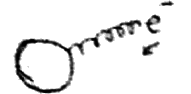
\includegraphics[width=0.2\textwidth]{./images/1-lorentz-model}
	\caption{Diagram of the Lorentz model for an atom}
	\label{fig:lorentz-model}
\end{figure}

Therefore, the equation of motion for the electron is
\begin{align*}
	\ddot{x} + \omega_{0}^{2}x = 0 \qc \omega_{0} = \sqrt{\frac{k}{m}} \Rightarrow x = A \cos(\omega_{0} t + \varphi)
\end{align*}
Introducing a damping term to account for the spontaneous emission, we get
\begin{align}
	\ddot{x} + \gamma \dot{x} + \omega_{0}^{2}x = 0
\end{align}

%-----------------------------------------------------------------
\subsection[Electric dipole approximation]{Electric dipole approximation (EDA)}
In the presence of an external electric field, $\va{E}(z,t) = E_{0} \cos(kz - \omega t) \vu{x}$, and introducing the oscillator strength, $f$, we can explain absorption and stimulated emission as well.

\begin{defi}[Oscillator strength]
	The oscillator strength, $f$, is a dimensionless quantity that expresses the probability of absorption or emission of electromagnetic radiation in transitions between energy levels of an atom or molecule.
	\begin{align*}
		f &> 0 \Rightarrow \text{ absorption} \\
		f &< 0 \Rightarrow \text{ stimulated emission}
	\end{align*}
\end{defi}

The force that acts upon a charged particle in the presence of an electric field is $\va{F} = q \va{E}$, therefore, we get
\begin{align*}
	\ddot{x} + \gamma \dot{x} + \omega_{0}^{2}x = f \frac{e E_{0}}{m} \cos(kz - \omega t)
\end{align*}

We can assume that the size of the atom is much smaller than the optical wavelength, so that the electron only sees the field at the nuclear position; this approximation is the so called electric dipole approximation. Therefore, $k z_{cm} \to 0$, and the previous equation becomes
\begin{align}
	\ddot{x} + \gamma \dot{x} + \omega_{0}^{2}x = f \frac{e E_{0}}{m} \cos(\omega t)
\end{align}

Consequently, we can get absorption or stimulated emission. Since $\dv*{W}{t} = - P$, we can study them measuring the mean value of the power in a cycle:
\begin{align}
	\ev{P} = \ev{F \dot{x}}
	\begin{cases}
		>0 & \text{(absorption)} \\
		<0 & \text{(stimulated emission)}
	\end{cases}
\end{align}
This models gives us $x(t)$.

\subsubsection*{Susceptibility}
In a homogeneous linear and isotropic dielectric medium, the polarization is aligned with and proportional to the electric field: $\va{P} = \varepsilon_{0} \chi \va{E}$. In a dipole, it can be written as $P = N e x$. Therefore, we can express the susceptibility as
\begin{align}
	\chi = \frac{N e x}{\varepsilon E} \equiv \chi' + i \chi''
\end{align}
The real part of the susceptibility, $\Re{\chi} = \chi'$ is related to index of refraction of the medium; the imaginary part, $\Im{\chi} = \chi''$ is related to the absorption coefficient.

\subsubsection*{Other media}
The natural frequency, $\omega_{0}$, gives us the model of the properties of the media. For metals, for instance, $\omega_{0} \to 0$ (electrons are not bound).

%-----------------------------------------------------------------
\subsection{Classical coherence}
\subsubsection*{First-order correlation function}
We can measure the coherence of an electric field with the help of an interferometer. In the figure \ref{fig:interferometer}, we see that $\va{E}_{1} = \va{E}(t)$, $\va{E}_{2} = \va{E}(t + \tau)$, and $\va{E}_{sum} = \va{E}_{1} + \va{E}_{2}$. So that, the intensity detected is $I \propto \ev{\va{E}^{2}_{sum}}$.
\begin{figure}[H]
	\centering
	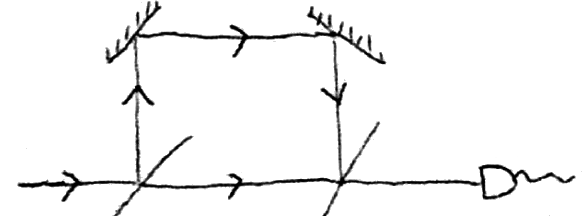
\includegraphics[width=0.5\textwidth]{./images/1-interferometer}
	\caption{Diagram of an interferometer with 50--50 beam splitters}
	\label{fig:interferometer}
\end{figure}

If we express $\va{E}(\va{r},t) = \va{E}^{(-}(\va{r},t) + \va{E}^{(-}(\va{r},t)$, where $\va{E}^{(+)} \equiv \va{E}^{(-)\sast}$, we can rewrite the expression for $I$:
\begin{flalign*}
	I & \propto \ev{(\va{E}_{1} + \va{E}_{2})^{2}} = \cdots = \ev{E^{(-)}_{1} E^{(+)}_{1}} + \ev{E^{(-)}_{2} E^{(+)}_{2}} + 2 \Re{ \ev{E^{(-)}_{1} E^{(+)}_{2}} } & \\
	& \Rightarrow I \propto 2 I_{0} + 2 \Re{E^{(-)}(t) + E^{(+)}(t + \tau)}
\end{flalign*}

\begin{defi}[First-order correlation function]
	\begin{align}
		G^{(1)}(t, t + \tau) \equiv \ev{E^{(-)}(t) + E^{(+)}(t + \tau)} = G^{(1)}(\tau)
	\end{align}
\end{defi}

The visibility is defined as $V = \dfrac{I_{max} - I_{min}}{I_{max} + I_{min}}$. Rewriting the first-order correlation function as $G^{(1)}(\tau) = \abs{G^{(1)}(\tau)} e^{i \phi(\tau)}$, we can easily work out $I_{max}$ and $I_{min}$:
\begin{flalign*}
	I & \propto 2 I_{0} + 2 \abs{G^{(1)}(\tau)} \cos[\phi(\tau)] \Rightarrow
	\begin{cases}
		I[\cos(\phi)] = -1 \Leftrightarrow I_{min} = 2I_{0} - 2 \abs{G^{(1)}(\tau)} \\
		I[\cos(\phi)] = +1 \Leftrightarrow I_{max} = 2I_{0} + 2 \abs{G^{(1)}(\tau)}
	\end{cases}
	 &
\end{flalign*}

\begin{defi}[Normalised first-order coherence function]
	We can rearrange the terms of the visibility to express it in terms of the first-order coherence function:
	\begin{align*}
		V = \dfrac{\abs{G^{(1)}(\tau)}}{\ev{E^{(-)}(t) E^{(+)}(t)}}
	\end{align*}
	this is what we call the normalised first-order coherence function, $g^{(1)}(\tau)$.
	\begin{align}
		V = \frac{I_{max} - I_{min}}{I_{max} + I_{min}} = \abs{g^{(1)}(\tau)}
		\begin{cases}
			= 0 & \Rightarrow \text{incoherent field} \\
			\in (0,1) & \Rightarrow \text{partially coherent field} \\
			= 1 & \Rightarrow \text{fully coherent field}
		\end{cases}
	\end{align}
\end{defi}

\subsubsection*{Second-order correlation function}
\begin{defi}[Normalised second-order correlation function]
	The degree of second-order correlation function is the autocorrelation function for the intensity, rather than the field. We can define this function as
	\begin{align}
		g^{(2)}(\tau) = \frac{\ev{ E^{(-)}(t) E^{(-)}(t + \tau) E^{(+)}(t + \tau) E^{(+)}(t) }}{\ev{ E^{(-)}(t) E^{(+)}(t) }}
	\end{align}
\end{defi}

%-----------------------------------------------------------------
\subsection{Hanbury--Brown--Twiss experiment}
One important feature of the second-order coherence function is that it can be measured with a reasonably simple set-up, the famous Hanbury--Brown–-Twiss apparatus (figure \ref{fig:hbt-experiment}). An input field is divided by a beam splitter, and the two components are monitored by two photo-detectors. The two detector signals are fed into a signal multiplier (mixer), though only after a variable time delay is added to one of the signals. The mixer signal is fed through a low-pass filter, which can be thought of as a integrator with a running time average.
\begin{figure}[H]
	\centering
	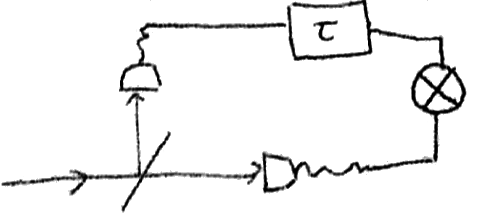
\includegraphics[width=0.4\textwidth]{./images/1-hbt-experiment}
	\caption{Diagram fo the Hanbury--Brown--Twiss experiment}
	\label{fig:hbt-experiment}
\end{figure}
This set-up, because it effectively correlates the two intensities, seems to give the $g^{(2)}(\tau)$ function as its output signal directly:
\begin{align}
	g^{(2)}(\tau) = \frac{\ev{I(t) I(t + \tau)}}{\ev{I(t)}^{2}}
\end{align}

\begin{align*}
	g^{(2)}(\tau)
	\begin{cases}
		\text{stationary field} & g^{(2)} (\tau) = 1 \\
		\text{fluctuating field} &
		\begin{cases}
			g^{(2)} (0) \geq 1 \\
			g^{(2)} (\tau) \leq g^{(2)} (0)
		\end{cases}
		\Rightarrow \text{bunching}
	\end{cases}
\end{align*}

\begin{figure}[H]
	\centering
	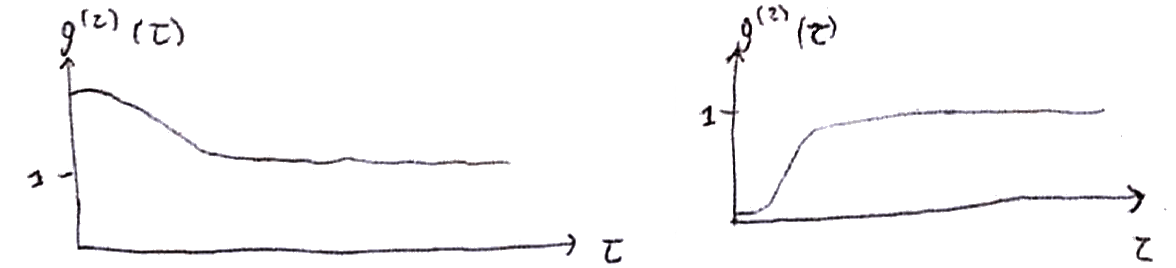
\includegraphics[width=\textwidth]{./images/1-bunching}
	\caption{(a) Bunching in a classical field, (b) antibunching in a quantum field}
	\label{fig:bunching}
\end{figure}

    %----------------------------------------------------------------------------------------
%    EQUACIONS DIFERENCIALS DE PRIMER ORDRE
%----------------------------------------------------------------------------------------
\section{Equacions diferencials de primer ordre}
\subsection{Equacions homogènies}
\subsubsection*{Funció homogènia}
\begin{defi}
$F(x,y)$ és homogènia de grau $n \Leftrightarrow F(tx, ty) = t^{n} F(x,y)$, $\quad \forall t$.
\end{defi}
Propietats:
\begin{enumerate}[i)]
    \item Si $F(x,y)$ és homogènia de grau $n$ i $G(x,y)$ és homogènia de grau $m$, llavors $FG$ i $\displaystyle \frac{F}{G}$ són homogènies de grau $n+m$ i $n-m$ respectivament.
    \item Si $F(x,y)$ és de grau zero, llavors $F(x,y)$ és funció únicament de $\displaystyle \frac{y}{x}$.
\end{enumerate}

\subsubsection*{Equació diferencial homogènia}
\begin{defi}
\begin{align}
    M(x,y) \diff x + N(x,y) \diff y = 0
\end{align}
amb $M$, $N$ homogènies del mateix grau.
\end{defi}

\subsubsection*{Resolució}
Es resolen per separació de variables.
\begin{example}
    $\displaystyle \frac{\dif y}{\dif x} = - \frac{M(x,y)}{N(x,y)} = f \left( \frac{y}{x} \right)$ i fent $y = vx$, $\displaystyle v + \frac{\dif v}{\dif x} x = f(v)$

    $\Rightarrow \boxed{\frac{\dif x}{x} = \frac{\dif v}{f(v) - v}}$.
\end{example}

\subsubsection*{Representació gràfica}
\begin{defi}[Homotècia]
$(x,y) \mapsto (kx, ky)$.
\end{defi}
Les corbes integrals es transformen unes en altres mitjançant homotècia.
\begin{example}
 $\displaystyle \frac{\dif y}{\dif x} = - \frac{x^{2} + y^{2}}{2x^{2}} = - \frac{1}{2} - \frac{y^{2}}{2x^{2}}$, funció només de $\displaystyle \frac{y}{x}$. Llavors, fem $\displaystyle v = \frac{y}{x}$ i separem $x, v$: $\displaystyle \frac{\dif v}{- \frac{1}{2} - \frac{v^{2}}{2} - v} = \frac{\dif x}{x} \Rightarrow - \frac{2 \diff v}{(1+v)^{2}} = \frac{\dif x}{x} \Rightarrow \ln x = \frac{2}{1+v} + C$

 $\Rightarrow \boxed{y = \left( \frac{2x}{\ln x + C} - x \right)}$.
\end{example}
\begin{example}
    $\displaystyle ky = \frac{2kx}{\ln kx + C} - kx \Rightarrow \boxed{y = \frac{2x}{\ln k + \ln x - C} - x} \Rightarrow$ fent $C' = C - \ln k$, obtenim una altra corba de la família.
\end{example}
%----------------------------------------------------------------------------------------
\subsection{Equacions lineals}
\begin{defi}
\begin{align}\label{ed-lineal}
   \frac{\dif y}{\dif x} + P(x) y = Q(x)
\end{align}
\end{defi}

\subsubsection*{Resolució}
Observem que $\displaystyle \frac{\dif}{\dif x} \left( y e^{\int P(x) \diff x} \right) = e^{\int P(x) \diff x} \left( \frac{\dif y}{\dif x} + y P(x) \right)$.

A partir de \eqref{ed-lineal} tenim: $\displaystyle e^{\int P(x) \diff x} \left( \frac{\dif y}{\dif x} + P(x) y \right) = Q(x) e^{\int P(x) \diff x}$. Integrant: $\displaystyle y e^{\int P(x) \diff x} = \int Q(x) e^{P(x) \diff x} \diff x + C \Rightarrow$
\begin{align}
    \boxed{y = C e^{-\int P(x) \diff x} + e^{-\int P(x) \diff x} \int Q(x) e^{\int P(x) \diff x} \diff x}
\end{align}

\begin{example}
	$\displaystyle x y' + (1 - x) y = e^{2x}$.

	$\displaystyle \Rightarrow P(x) \equiv \frac{1 - x}{x}, \, Q(x) = \frac{e^{2x}}{x} \Rightarrow \int P(x) \diff x = \ln x - x \Rightarrow y = C \frac{e^{x}}{x} + \frac{e^{x}}{x} \int \frac{x e^{-x}}{x} e^{2x} \diff x$

	$\Rightarrow \boxed{y = C \frac{e^{x}}{x} + \frac{e^{2x}}{x}}$.
\end{example}

\subsubsection*{Propietats de les solucions de l'equació diferencial de 1r ordre}
\begin{enumerate}[i)]
	\item Si $y_{1}$ és una solució particular de la reduïda, la solució general de la reduïda és $y = C y_{1}$.
	\item Si $y_{1}$ és una solució particular de la reduïda i $y_{2}$ una solució particular de la completa, llavors la solució general de la completa és $y = C y_{1} + y_{2}$.
	\item Si $y_{1}$, $y_{2}$ són dues solucions particulars diferents de la completa, la solució general de la completa és $y = y_{2} + C(y_{2} - y_{1})$.
\end{enumerate}
\begin{example}
	$y' + y = 10$, amb una solució particular de la reduïda $y = e^{-x}$; de la completa $y = 10$. Llavors, $\boxed{y = C e^{-x} + 10}$.
\end{example}
\begin{example}
	$\displaystyle y' + \frac{y}{x^{2}} = 2x + 1$, amb una solució particular de la completa $y = x^{2}$. Llavors, $\boxed{y = C e^{\sfrac{1}{x}} + x^{2}}$.
\end{example}

%----------------------------------------------------------------------------------------
\subsection{Equació de Bernoulli}
\begin{defi}
	\begin{align}
		\frac{\dif y}{\dif x} + P(x) y = Q(x) y^{n}
	\end{align}
\end{defi}

\subsubsection*{Resolució}
Aquesta ED ja és lineal per a $n = 0$ i $n = 1$. A la resta de casos, es pot linealitzar amb el canvi de variable $\boxed{z = y^{1-n}}$.

Tenim $\displaystyle \frac{\dif z}{\dif x} = (1-n) y^{-n} \frac{\dif y}{\dif x}$, i l'ED queda: $\displaystyle y^{-n} \frac{\dif y}{\dif x} + P(x) y^{1-n} = Q(x) \Rightarrow$
\begin{align}
    \boxed{\frac{\dif z}{\dif x} + (1-n) P(x) z = (1-n) Q(x)}
\end{align}
\begin{example}
	$\displaystyle \frac{\dif y}{\dif x} + \frac{y}{x} = y^{2} \frac{x \cos x - \sin x}{x}$.

	És una equació de Bernoulli amb $\displaystyle n = 2 \Rightarrow z = \frac{1}{y}$. Llavors, queda $\displaystyle \frac{\dif z}{\dif x} - \frac{z}{x} = \frac{\sin x - x \cos x}{x}.$

	Resolem l'ED lineal: $\displaystyle P(x) = - \frac{1}{x} \Rightarrow e^{- \int P(x) \diff x} = x \Rightarrow z = Cx + x \int \frac{\sin x - x \cos x}{x^{s}} \diff x = Cx - \sin x \Rightarrow \boxed{y = \frac{1}{Cx - \sin x}}$
\end{example}

%----------------------------------------------------------------------------------------
\subsection{Equació de Ricatti}
\begin{defi}
	\begin{align}
		\frac{\dif y}{\dif x} = P(x) y^{2} + Q(x) y + R(x)
	\end{align}
\end{defi}
\subsubsection*{Resolució}
És una ED no resoluble en general, però sí a partir d'una solució particular $y_{p}$. Sigui $\displaystyle y_{p}' = P(x) y^{2}_{p} + Q(x) y_{p} + R(x)$.

Cerquem $\boxed{z = y - y_{p}} \Rightarrow z' = Pz (y + y_{p}) + Qz \Leftrightarrow$
\begin{align}
    \boxed{z' - (2y_{p} P + Q)z = Pz^{2}}
\end{align}
que és una equació de Bernoulli amb $n = 2$, que es resol amb el canvi $\displaystyle w = \frac{1}{z}$.
\begin{example}
	$\displaystyle y' = x^{3} (y-x)^{2} + \frac{y}{x}$, amb $y_{p} = x$.

	Tenim $P(x) = x^{3}$, $\displaystyle Q(x) = -2x^{4} + \frac{1}{x}$, $R(x) = x^{5}$.
	\begin{enumerate}[i)]
		\item Ricatti $\mapsto$ Bernoulli:
			\subitem $\displaystyle z = y - x \Rightarrow z' - \left(2x^{4} - 2x^{4} + \frac{1}{x} \right) z  = x^{3} z^{2} \Rightarrow z' - \frac{z}{x} = x^{3} z^{2} \Rightarrow P = - \frac{1}{x}, \, Q = x^{3}, \, n=2$.
		\item Bernoulli $\mapsto$ lineal:
			\subitem $\displaystyle w = \frac{1}{z} \Rightarrow w' + \frac{w}{x} = -x^{3}$.
			\subitem Resolem: $\displaystyle \Rightarrow w = \frac{C}{x} - \frac{x^{4}}{5}$.
		\item Retorn $w \mapsto z \mapsto y$.
			\subitem $\boxed{y = \frac{5x}{5C - x^{5}}}$.
	\end{enumerate}
\end{example}

%----------------------------------------------------------------------------------------
\subsection{Equacions exactes}
\begin{defi}
	\begin{align}
    \begin{gathered}
		M(x,y) \diff x + N(x,y) \diff y = 0 \text{ és exacta} \Leftrightarrow \\
        \exists f(x,y) \mid \dif f \equiv M \diff x + N \diff y
    \end{gathered}
	\end{align}
\end{defi}
\begin{thm}[d'Euler]
	Una ED de la forma $M(x,y) \diff x + N(x,y) \diff y = 0$ és exacta si i només si $\displaystyle \frac{\partial M}{\partial y} = \frac{\partial N}{\partial x}$.
\end{thm}

\subsubsection*{Resolució}
Si l'ED és exacta, llavors $\dif f = 0$. Així doncs,
\begin{align}
    \boxed{f(x,y) \equiv C = \int_{a}^{x} M(x,y) \diff x + \int N(a,y) \diff y}
\end{align}
Alternativament, podem considerar el següent: $\displaystyle f = \int M(x,y) \diff x + g(y)$ i $\displaystyle g'(y) \equiv N(x,y) - \frac{\partial}{\partial y} \left( \int M(x,y) \diff x \right)$. Llavors,
\begin{align}
	\boxed{C = \int M \diff x + \int \left( N - \frac{\partial}{\partial y} \int M \diff x \right) \diff y}
\end{align}

\begin{example}
	$\displaystyle \left( \frac{y}{x} + y^{3} \right) \diff x + \left( \ln x + 3x y^{2} + 4y \right) \diff y = 0$.

	Comprovem que sigui exacta: $\displaystyle \frac{\partial M}{\partial y} = \frac{1}{x} + 3y^{2} = \frac{\partial N}{\partial x} = \frac{1}{x} + 3y^{2}$.

	Tenim  $\displaystyle f(x,y) = \int_{a}^{x} M(x,y) \diff x + \int N(a,y) \diff y \Rightarrow f = y \ln x + x y^{3} + 2y^{2}$. La solució és $\boxed{y \ln x + x y^{3} + 2y^{2} = C}$.

    Altrament podem fer $f = y \ln x + xy^{3} + g(y) \Rightarrow g'(y) = \ln x + 3xy^{2} + 4y - \ln x  3xy^{2} = 4y \Rightarrow g(y) = 2y^{2}$. La solució és $\boxed{y \ln x + x y^{3} + 2y^{2} = C}$.
\end{example}

%----------------------------------------------------------------------------------------
\subsection{Factors integrants}
\begin{defi}
	Una funció $\mu(x,y)$ és factor integrant de l'equació $M \diff x + N \diff y = 0 \Leftrightarrow$
	\begin{align}
		\mu M(x,y) \diff x + \mu N(x,y) \diff y = 0 \text{ és exacta}
	\end{align}
\end{defi}
\begin{example}
	$2y \diff x + x \diff y = 0$ no és exacta, però agafant $\mu = x \Rightarrow 2xy \diff x + x^{2} \diff y = 0$ és exacta.
\end{example}
Propietat: $\exists$ sempre una infinitat de factors integrants. Ja que $\exists$ una solució $f(x,y) = C$, es té $\displaystyle \frac{\partial f}{\partial x} \diff x + \frac{\partial f}{\partial y} \diff y = 0$. Llavors, només cal fer:
\begin{align}
	\boxed{\mu = \frac{\partial f / \partial x}{M} = \frac{\partial f / \partial y}{N}}
\end{align}
\begin{example}
	Per a $2y \diff x + x \diff y = 0$, qualsevol factor de la forma $x F(x^{2}y)$ és factor integrant.
\end{example}

\subsubsection*{Mètode per trobar $\mu$}
Segons convingui s'ha de trobar una funció $G$ o una funció $H$ tal que $e^{\int G}$ o $e^{\int H}$ sigui factor integrant.
\begin{align}
	\boxed{G \equiv \frac{1}{N} \left( \frac{\partial M}{\partial y} - \frac{\partial N}{\partial x} \right) \Rightarrow \mu = \mu = e^{\int G}}
\end{align}
\begin{align}
	\boxed{H \equiv \frac{1}{M} \left( \frac{\partial N}{\partial x} - \frac{\partial M}{\partial y} \right) \Rightarrow \mu = \mu = e^{\int H}}
\end{align}
\begin{example}
	$(4x^{2} + y) \diff x - x \diff y = 0$ no exacta.

	$\displaystyle G = - \frac{1}{x} (1 - (-1)) = - \frac{2}{x} \Rightarrow \mu = e^{-2 \ln x} = \frac{1}{x^{2}}$

	Resolent la nova equació exacta, obtenim: $\boxed{4x - \frac{y}{x} = C}$.
\end{example}
%----------------------------------------------------------------------------------------
\subsection{Equacions de 2n ordre resoltes per mètodes de 1r ordre}
Les ED de la forma $\displaystyle f \left( x, y, \frac{\dif y}{\dif x}, \frac{\dif^{2} y}{\dif x^{2}} \right) = 0$ es resol per mètodes de 1r ordre ens dos casos:
\begin{enumerate}[i)]
	\item $\displaystyle f \left( x, \frac{\dif y}{\dif x}, \frac{\dif^{2} y}{\dif x^{2}} \right) = 0$, només cal fer el canvi $\displaystyle v = \frac{\dif y}{\dif x}$.
	\item $\displaystyle f \left( y, \frac{\dif y}{\dif x}, \frac{\dif^{2} y}{\dif x^{2}} \right) = 0$, només cal fer el canvi $\displaystyle v = \frac{\dif y}{\dif x}$ i $\displaystyle v \frac{\dif v}{\dif y} = \frac{\dif^{2} y}{\dif x^{2}}$.
\end{enumerate}
\begin{example}
	$\displaystyle y \frac{\dif^{2} y}{\dif x^{2}} = 2 \left( \frac{\dif y}{\dif x} \right)^{2}$.

	Fent els canvis de variable, tenim $\displaystyle y v \frac{\dif v}{\dif y} = 2v^{2}$. Separant les variables i integrant, obtenim $2 \ln y = \ln v + A$. Fent $\ln B = A$ i desfent els logaritmes tenim $y^{2} = Bv$.

	Desfem el canvi de variable i obtenim $\displaystyle y^{2} = B \frac{\dif y}{\dif x} \Rightarrow \dif x = B \frac{\dif y}{y^{2}} \Rightarrow x = - \frac{B}{y} + C \Rightarrow y = - \frac{B}{x-C} \Rightarrow \boxed{y = \frac{1}{C_{1} x + C_{2}}}$.
\end{example}

%----------------------------------------------------------------------------------------
\subsection{Equació de Clairaut}
\begin{defi}
	Sigui la família de rectes no paral·leles a un paràmtre.
	\begin{align}
		y = Cx + f(C)
	\end{align}
	L'ED més general que compleix aquesta solució és la que s'obté fent $\displaystyle \frac{\dif y}{\dif x} = C$:	\begin{align}
		y = \frac{\dif y}{\dif x} x + f\left( \frac{\dif y}{\dif x} \right)
	\end{align}
\end{defi}

\begin{example}\label{sol-sing}
	$\displaystyle y = x \frac{\dif y}{\dif x} - \frac{1}{4} \left( \frac{\dif y}{\dif x} \right)^{2}$. La solució és $\boxed{y = Cx - \frac{1}{4} C^{2}}$.
\end{example}
\begin{example}
	$\displaystyle y = x \frac{\dif y}{\dif x} - \frac{\dif x}{\dif y}$. La solució és $\boxed{y = Cx - C^{-1}}$.
\end{example}
\begin{example}
	$\displaystyle \left(y - x \frac{\dif y}{\dif x} \right) + \frac{\dif y}{\dif x} = \left( \frac{\dif y}{\dif x} \right)^{2}$.

    La solució és $\boxed{y = Cx \pm \sqrt{C^{2} - C}}$.
\end{example}

\begin{defi}[Solució singular]
	És una solució adicional de l'ED, no inclosa en la solució general.
\end{defi}
\begin{example}
	A l'equació de l'exemple~\ref{sol-sing}, $\boxed{y = x^{2}}$ és una solució singular.
\end{example}

\subsubsection*{Corba envolvent}
\begin{defi}
	És una corba tangent en cadascun dels seus punts a alguna de les rectes. Si $\exists$ l'envolvent, aquesta és solució de l'ED.
\end{defi}
Una condició necessària de l'envolvent és que $\displaystyle x = - \frac{\dif f(C)}{\dif C}, \quad \forall x$. Com que l'envolvent també verifica $y = Cx + f(C)$, l'envolvent s'obté aïllant $C$ a les dues equacions.
\begin{example}
	$y = Cx - C^{-1}$.

	$\displaystyle x = \frac{\dif}{\dif C} (C^{-1}) = - C^{-2} \Rightarrow C^{2} = -x^{-1}$.

	Pel binomi de Newton $\Rightarrow y^{2} = C^{2} x^{2} - 2x + C^{-2} \Rightarrow \boxed{y^{2} = -4x}$ és l'envolvent.
\end{example}
\begin{example}[amb dues envolvents]
	$\displaystyle y = \frac{\dif y}{\dif x} x - \frac{1}{3} \left( \frac{\dif y}{\dif x} \right)^{3} \Rightarrow$

    $\boxed{y = Cx - \frac{1}{3} C^{3}}$ és la solució general, però $\boxed{y = \pm x^{\sfrac{3}{2}}}$ són dues solucions singulars.
\end{example}
Observació: les solucions que trobem per aquest mètode són candidats a envolvents; s'ha de comprovar directament a l'ED per substitució.

%----------------------------------------------------------------------------------------
\subsection{Família de corbes a $n$ paràmetres}
\begin{defi}
	Una relació de la forma $F(x,y,C_{1}, \dots, C_{n}) = 0$ representa una família de corbes a $n$ paràmetres. Satisfan una ED d'ordre $n$ (si els $n$ paràmetres són essencials), la qual s'obté derivant $n$ vegades, és a dir, fins a $\displaystyle F(x,y,C_{1}, \dots, C_{n}, \frac{\dif y}{\dif x}, \dots , \frac{\dif^{n} y}{\dif x^{n}})$ i eliminant $C_{1}, \dots , C_{n}$ entre aquestes $n+1$ relacions.
\end{defi}
\begin{example}
	ED de tots els cercles de radi unitat: $(x-a)^{2} + (y-b)^{2} = 1$.
	\begin{enumerate}[i)]
	    \item $\displaystyle 2(x-a) \diff x + 2 (y-b) \diff y = 0 \Rightarrow x-a = (b-y) \frac{\dif y}{\dif x}$.
	    \item $\displaystyle 1 = -1 \left( \frac{\dif y}{\dif x} \right)^{2} + (b-y) \frac{\dif^{2} y}{\dif x^{2}} \Rightarrow y-b = \frac{1+y'^{2}}{-y''}$.
	    \item Substituint l'ED del pas i) a l'equació del cercle, obtenim $\displaystyle (y-b)^{2} \left[ 1 + \left( \frac{\dif y}{\dif x} \right) \right]$.
	    \item Finalment, considerant els resultats dels passos ii) i iii), obtenim $\boxed{(1 + y'^{2})^{3} = y''^{2}}$.
	\end{enumerate}
	Observem, llavors, que el radi de curvatura d'una corba és $\boxed{\frac{(1 + y'^{2})^{\sfrac{3}{2}}}{|y''|}}$.
\end{example}

    %----------------------------------------------------------------------------------------
%    EQUACIONS DIFERENCIALS LINEALS
%----------------------------------------------------------------------------------------
\section{Equacions diferencials lineals}
\subsection{Equacions reduïdes i completes}
\begin{defi}[Equació diferencial d'ordre $n$]
    \begin{align}\label{ed-lineal-n}
        \frac{\dif^{n} y}{\dif x^{n}} + P_{1}(x) \frac{\dif^{n-1} y}{\dif x^{n-1}} + \cdots + P_{n-1}(x) \frac{\dif y}{\dif x} + P_{n}(x) y = R(x)
	\end{align}
	\begin{itemize}
		\item Si $R(x) = 0$, es tracta d'una ED reduïda.
		\item Si $R(x) \neq 0$, es tracta d'una ED completa.
	\end{itemize}
\end{defi}

\subsubsection*{Propietats de les equacions reduïdes i completes}
\begin{enumerate}[i)]
    \item Si una solució de la reduïda s'anul·la, al igual que les seves $n-1$ derivades en algun punt $x_{0}$, aquesta solució és $y(x) \equiv 0$.
	\item Si $u_{1}, \dots , u_{k}$ són solucions de la reduïda, també ho són $Cu_{1}, \dots , Cu_{k}$.
	\item Si $y_{1}, y_{2}$ són solucions de la completa, $y_{2} - y_{1}$ és solució de la reduïda.
\end{enumerate}
\begin{cor}
    Si $y_{1}$ és una solució particular de la completa, i $u_{1}$ la solució general de la reduïda, llavors $y_{1} + u_{1}$ és la solució general de la completa.
\end{cor}
Sabem per resultats de capítols anteriors que:
\begin{itemize}
	\item Solució general d'una ED d'ordre $n$: funció $y(x)$ amb $n$ constants arbitràries.
	\item $\exists! y(x)$ amb valors predeterminats per a $y(x_{0}), y'(x_{0}), \dots , y^{(n-1)}(x_{0})$.
\end{itemize}

\begin{thm}
	La solució general d'una ED lineal completa s'obté sumant la solució general de la reduïda i una solució particular de la completa.
\end{thm}
\begin{defi}[Wronskià]
	\begin{align}
		W(u_{1}(x), \dots , u_{n}(x)) \equiv \begin{vmatrix} u_{1} & \dots & u_{n} \\ u'_{1} & \dots & u'_{n} \\ \vdots & & \vdots \\ u^{(n-1)}_{1} & \dots & u^{(n-1)}_{n} \end{vmatrix} \equiv f(x)
	\end{align}
\end{defi}
\begin{thm}
	Si $n$ funcions són linealment dependents (LD) i $\exists$ les seves derivades fins a $n-1$, el seu wronskià és $\equiv 0$.
\end{thm}
\begin{thm}
	Tota solució de l'ED reduïda es pot expressar com a combinació lineal de $n$ solucions linealment independents (LI) de la reduïda.
\end{thm}
\begin{cor}
	La forma de trobar la solució general de l'ED reduïda és trobar $n$ solucions particulars LI (mitjançant el wronskià és fàcil comprovar si ho són).
\end{cor}

%----------------------------------------------------------------------------------------
\subsection{Equacions reduïdes amb coeficients constants}
\begin{defi}
	\begin{align}\label{ed-red-ct-n}
		\frac{\dif^{n} y}{\dif x^{n}} + p_{1} \frac{\dif^{n-1} y}{\dif x^{n-1}} + \dots + p_{n-1} \frac{\dif y}{\dif x} + p_{n} y = 0
	\end{align}
\end{defi}

\subsubsection*{Resolució}
\begin{defi}[Equació auxiliar]
	$\exists$ solucions de l'ED~\eqref{ed-red-ct-n} de la forma $y = e^{mx}$ on $m$ és arrel de l'equació auxiliar $m^{n} + p_{1} m^{n-1} + \dots + p_{n-1} m + p_{n} = 0$.
\end{defi}
Segons com siguin les arrels de l'equació auxiliar, tindrem diferents solucions:
\begin{enumerate}[i)]
	\item Si són $n$ arrels reals diferents: $m_{1}, \dots , m_{n}$.
		\subitem $\Rightarrow \boxed{y = C_{1}e^{m_{1}x} + \dots + C_{n}e^{m_{n}x}}$ és solució.
	\item Si són $n$ arrels reals, però alguna múltiple: $m_{k}$ amb multiplicitat $r$.
		\subitem Se substitueixen els $r$ sumands amb $e^{m_{k}x}$ de la solució anterior per
		\subitem $\boxed{(B_{1} + B_{2} x + \dots + B_{r} x^{r-1}) e^{m_{k}x}}$.
	\item Si hi ha alguna arrel complexa: $m = \alpha \pm \beta \imath$.
		\subitem Se substitueixen els termes $C e^{(\alpha + \beta \imath) x} + D e^{(\alpha + \beta \imath) x}$ per $\boxed{e^{\alpha x} (A \cos \beta + B \sin \beta)}$.
	\item Si hi ha alguna arrel complexa múltiple: $m_{k} = \alpha \pm \beta \imath$ arrel de multiplicitat $r$
		\subitem Se substitueixen $2r$ termes de la primera solució per
		\subitem $\boxed{e^{\alpha x} \left[ (A_{1} + A_{2} x + \dots + A_{r} x^{r-1})\cos \beta x \right]}$
		\subitem $+ \boxed{e^{\alpha x} \left[ (B_{1} + B_{2} x + \dots + B_{r} x^{r-1})\sin \beta x \right]}$.
\end{enumerate}

\begin{example}
	$y'' + 4y' + 4y = x + 1 \Rightarrow m^2 + 4m + 4 = 0 \Rightarrow m = -2$ (doble).

	$\Rightarrow \boxed{y = e^{-2x} (A + Bx)}$ és solució de la reduïda.
\end{example}
\begin{example}
	$y^{(4)} + 5y'' + 4y = 0 \Rightarrow m^{4} + 5m^{2} + 4 = 0 \Rightarrow m_{1} = \pm \imath, m_{2} = \pm 2 \imath$.

	$\Rightarrow \boxed{y = A \cos x + B \sin x + C \cos 2x + D \sin 2x}$ és solució.
\end{example}

%----------------------------------------------------------------------------------------
\subsection{Equacions completes amb coeficients constants}
\begin{defi}
	\begin{align}\label{ed-comp-ct-n}
		\frac{\dif^{n} y}{\dif x^{n}} + p_{1} \frac{\dif^{n-1} y}{\dif x^{n-1}} + \dots + p_{n-1} \frac{\dif y}{\dif x} + p_{n} y = R(x)
	\end{align}
\end{defi}
\subsubsection*{Mètode dels anihiladors}
\begin{defi}
    Emprant la notació d'Euler ($y^{(n)} = D^{n}y$), l'equació~\eqref{ed-comp-ct-n} s'escriurà:
    \begin{align}
        L(y) = (D^{n} + p_{1} D^{n-1} + \dots + p_{n-1} D + p_{n}) y = R(x)
    \end{align}
    On $L$ és l'operador lineal diferencial $D^{n} + p_{1} D^{n-1} + \dots + p_{n-1} D + p_{n}$. És fàcil veure que $L = (D-m_{1}) (D-m_{2}) \dots (D-m_{n})$, on $m_{i}$ śon les arrels de l'equació auxiliar.
\end{defi}
\begin{defi}[Operador anihilador]
Un operador anihilador és un operador lineal $L_{i}$ que anihila $R(x)$, és a dir $L_{1} L_{2} \dots L_{k} R(x) = 0$.
\begin{itemize}
    \item $\boxed{(D-\alpha)^{n+1}}$ anihila les funcions que tenen forma de $\boxed{x^{n} e^{\alpha x}}$.
    \item $\boxed{(D^{2}-2\alpha D + \alpha^{2} + \beta^{2})^{n+1}}$ anihila les funcions que tenen forma de

    $\boxed{x^{n} e^{\alpha x} (C_{1} \cos \beta x + C_{2} \sin \beta x)}$.
\end{itemize}
\end{defi}
\subsubsection*{Resolució}
\begin{enumerate}[i)]
    \item Solucionar l'ED reduïda $L(y) = 0$.
    \item Multiplicar pels operadors anihiladors a ambdues bandes de l'ED:

    $L'(y) \equiv (L_{1}L_{2} \dots L)(y) = L_{1}L_{2} \dots R(x) \equiv 0$.
    \item Trobar les arrels de $L'$ i expressar solució general corresponent a l'equació $L'(y) = 0$.
    \item Els sumands de la solució de $L'(y) = 0$ que no siguin ja a la solució de la reduïda són la solució particular de la completa que busquem. És a dir, tenim $y_{p} = C_{1} P_{1}(x) + C_{2} P_{2}(x) + \dots$.
    \item Substituir $y$ de l'ED inicial per $y_{p}$, aplicar l'operador $L$ i trobar els valors de les constants $C_{i}$ per tal que es compleixi $L(y_{p}) = R(x)$.
\end{enumerate}
\begin{example}
    $y''' - y' = x e^{x} \Rightarrow (D^{3} - D) y = xe^{x}$

    Reduïda: $(D^{3} - D) = D (D-1) (D+1) = 0 \Rightarrow \boxed{y = A + Be^{x} + Ce^{-x}}$.

    L'operador que anihila $x e^{x}$ és $(D-1)^{2} \Rightarrow D (D-1)^{3} (D+1) = 0$. Llavors tenim $m_{1} = 0$, $m_{2} = 1$ (triple), $m_{3} = -1$. La solució general és $\boxed{y = (B + Ex + Fx^{2})e^{x} + A + Ce^{-x}}$.

    $\Rightarrow \boxed{y_{p} = Exe^{x} + Fx^{2} e^{x}} \Rightarrow (D^{3}-D) (Exe^{x} + Fx^{2} e^{x}) = xe^{x} = (2E + 6F)e^{x} + 4Fxe^{x}$.

    $\displaystyle \Rightarrow E = -\frac{3}{4}, F = \frac{1}{4} \Rightarrow \boxed{y_{p} = -\frac{3}{4} xe^{x} + \frac{1}{4} x^{2} e^{x}}$.
\end{example}

%----------------------------------------------------------------------------------------
\subsection{Mètode de la variació de paràmetres (2n ordre)}
En general és un mètode vàlid $\forall$ funció $R(x)$. A més no es limita al cas dels coeficients constants, sinó que és vàlid sempre que s'hagi resolt l'ED reduïda.
\begin{defi}
	\begin{align}\label{ed-var-par-2}
		y'' + P(x) y' + Q(x) y = R(x)
	\end{align}
\end{defi}

\subsubsection*{Resolució}
Siguin $u_{1}, u_{2}$ solucions LI de la reduïda ($u''_{i} + Pu'_{i} + Q_{i} = 0$). Cerquem una solució de la concreta de la forma
\begin{align*}
	y = t_{1}(x) u_{1} + t_{2}(x) u_{2}
\end{align*}
i, a més, compleix la següent propietat: $t'_{1}(x) u_{1} + t'_{2}(x) u_{2} = 0$.
\\
Derivant, substituint a~\eqref{ed-var-par-2}, tenim: $t'_{1}(x) u'_{1} + t'_{2}(x) u'_{2} = R \Rightarrow \exists t_{1}, t_{2} \mid y = t_{1}(x) u_{1} + t_{2}(x) u_{2}$. Així doncs, tenim el següent sistema d'equacions algebràiques:
\begin{align*}
	\begin{cases} t'_{1}(x) u_{1} + t'_{2}(x) u_{2} = 0 \\ t'_{1}(x) u'_{1} + t'_{2}(x) u'_{2} = R \end{cases}
\end{align*}
La solució del sistema és $\displaystyle t'_{1} = - \frac{Ru_{1}}{W}, t'_{2} = \frac{Ru_{2}}{W}$, on el wronskià val $W = u_{1} u'_{2} - u'_{1} u_{2}$. Integrant les $t'_{i}$ respecte $x$, tenim:
\begin{align}
	\boxed{y_{p} = - u_{1}(x) \int_{a}^{x} \frac{R(x) u_{2}(x)}{W(x)} \diff x + u_{2}(x) \int_{a}^{x} \frac{R(x) u_{1}(x)}{W(x)} \diff x}
\end{align}

\begin{example}
    $\displaystyle y'' + y = \frac{1}{\sin x}$. $m = \pm \imath$.
    La solució de la reduïda és $\boxed{y = A \cos x + B \sin x}$. Llavors definim $u_{1} = \cos x$ i $u_{2} = \sin x$.

    $W(u_{1}(x), u_{2}(x)) = \cos^{2} x + \sin^{2} x = 1 \neq 0$.

    $\displaystyle y_{p} = \cos x \int_{a}^{x} \frac{\sin x}{\sin x} \diff x + \sin x \int_{a}^{x} \frac{\cos x}{\sin x} \diff x$

    $y_{p} = \cos x (a-x) + \sin x \ln (\sin x) - \sin x (\ln (\sin a))$,

    però $a \cos x$ i  $\sin x (\ln (\sin a))$ s'absorveixen en la solució de la reduïda.

    Llavors, $\boxed{y_{p} = - x \cos x + \sin x \ln (\sin x)}$ és una solució particular de la completa.

    $\Rightarrow \boxed{y = A \cos x + B \sin x - x \cos x + \sin x \ln (\sin x)}$.
\end{example}

%----------------------------------------------------------------------------------------
%\subsection{Mètode de la variació de paràmetres (ordre $n$)} %WIP

%----------------------------------------------------------------------------------------
\subsection{Reducció de l'ordre d'una equació}
\subsubsection*{Equació lineal de 2n ordre}
Sigui $y'' + P(x) y' + Q(x) y = R(x)$ i sigui $u(x)$ no $\equiv 0$ una solució de la reduïda.

Fem el canvi de variable $\boxed{y = tu}$. Llavors $y' = tu' + t'u$, $y'' = tu'' + 2t'u' + t''u$.

Substituïm en l'ED completa: $t(u'' + Pu' + Qu) + t'(2u' + Pu) + t'' u = R$. Com que $u$ és solució de la reduïda, $u'' + Pu' + Qu = 0 \Rightarrow t(u'' + Pu' + Qu) + t'' u = R$ i fem el canvi de variable $\boxed{v = t'} \Rightarrow$
\begin{align}
    \boxed{v(2u' +P(x)u) + vu' = R(x)}
\end{align}
Llavors, determinem $v$, desfem el canvi per trobar $t$ i tornem a desfer el canvi per trobar la solució de $y(x)$.
\begin{example}
$x y'' - 2 (x + 1) y' + (x+2) y = x^{3} e^{2x}$, amb $u = e^{x}$.

$\displaystyle \Rightarrow v \left( 2 - 2 \frac{x + 1}{x} \right) + v' = x^{2} e^{x} \Rightarrow - \frac{2v}{x} + v' = x^{2} e^{x} \Rightarrow \frac{v' x^{2} - 2vx}{x^{4}} = e^{x} \Rightarrow e^{x} = \frac{\dif}{\dif x} \left( \frac{v}{x^{2}} \right) \Rightarrow \frac{v}{x^{2}} = e^{x} + C \Rightarrow \boxed{v = C x^{2} + x^{2} e^{x}}$

$\displaystyle t = (x^{2} - 2x + 2) e^{x} + \frac{C}{3} + D \Rightarrow \boxed{ y = \left[ (x^{2} - 2x + 2)e^{x} + \frac{C}{3} + D \right] e^{x}}$.
\end{example}
Altrament, si tenim $y'' + P(x) y' + Q(x) y = R(x)$ i $y_{1}(x)$ no $\equiv 0$ és una solució. Llavors, $y_{2} = y_{1} t$ és una altra solució linealment independent respecte $y_{1}$.

En particular, $\displaystyle y_{2} = y_{1} \int \frac{e^{-\int P(x) \diff x}}{y_{1}^{2}} \diff x$. I per tant, la solució general és $\boxed{y = C_{1}y_{1} + C_{2} y_{2}}$.
\begin{example}
    $\displaystyle y'' + \frac{1}{x} y' + \left( 1 - \frac{1}{4x^{2}} \right) y = 0$, amb solució $\displaystyle y_{1} = \frac{\sin x}{\sqrt{x}}$.

    $\Rightarrow \displaystyle y_{2} = y_{1} \int \frac{e^{-\int \frac{1}{x} \diff x}}{y_{1}^{2}} \diff x = - \frac{\cos x}{\sqrt{x}}$

    $\Rightarrow \boxed{y = C_{1} \frac{\sin x}{\sqrt{x}} + C_{2} \frac{\cos x}{\sqrt{x}}}$ és la solució general de l'ED (notem que el signe negatiu de $y_{2}$ ja el conté la constant).
\end{example}

%\subsubsection*{Equació d'ordre $n$} %WIP
%Sigui una ED reduïda d'ordre $n$:
%\begin{align}\label{ed-reduc-n}
%    	y^{(n)} + y^{(n-1)} P_{1}(x) + \dots + P_{n}(x) y = 0
%\end{align}
%\begin{thm}
%    Si es coneixen $u_{1}(x), \dots u_{p}(x)$ LI, l'equació~\eqref{ed-reduc-n} es pot reduir a una equació d'ordre $n-p$ en la variable $v$.
%    \begin{align*}
%        v = \begin{vmatrix} u_{1} & \dots & u_{p} & y \\  \vdots & &  & \vdots \\ u_{1}^{(p)} & \dots & u_{p}^{(p)} & y^{(p)} \end{vmatrix} \phi(x)
%    \end{align*}
%    on $\phi(x)$ és una funció arbitrària.
%\end{thm}

%\subsubsection*{Casos}
%1) Es coneix $u(x)$ no $\equiv 0$.

%$v = \begin{vmatrix} u & y \\ u' & y' \end{vmatrix} \phi(x)$, convé fer $\displaystyle \phi(x) = \frac{1}{u(x)^{2}}$.

%$v = \left( \frac{y}{u} \right)' \Rightarrow y = tu$ amb $t' = v$.

%----------------------------------------------------------------------------------------
\subsection{Equació de Cauchy-Euler}
\begin{defi}
\begin{align}
    x^{2} \frac{\partial^{2} y}{\partial x^{2}} + px \frac{\partial y}{\partial x} + qy = R(x)
\end{align}
\end{defi}
Es redueix a una de coeficients constants amb el canvi de variable $x= e^{t}$ o $t = \ln x$. Així doncs, per la regla de la cadena, l'equació queda
\begin{align}
    \frac{\partial^{2} y}{\partial t^{2}} - \frac{\partial y}{\partial t} + p \frac{\partial y}{\partial t} + qy = R(t)
\end{align}

\begin{example}
    $x^{2}y'' -4y' +6y = 2x + 5$ queda, fent el canvi $x = e^{t}$, $y'' -5 y' + 6y = 2e^{t} + 5$.

    $\displaystyle \Rightarrow \boxed{y = Ae^{2t} + Be^{3t} + e^{t} + \frac{5}{6}}$.
\end{example}

%----------------------------------------------------------------------------------------
\subsection{Equacions exactes de 2n ordre}
\begin{defi}
    \begin{align}
        P_{2}(x) \frac{\dif^{2} y}{\dif x^{2}} + P_{1}(x) \frac{\dif y}{\dif x} + P_{0} y = R(x)
    \end{align}
\end{defi}
\begin{thm}
    Una ED de segon ordre és exacta $\Leftrightarrow P_{2}''(x) - P_{1}'(x) + P_{0}(x) \equiv 0$.
\end{thm}
\subsubsection*{Resolució}
Per a les equacions exactes de segon ordre hi haurà prou amb resoldre una equació lineal de primer ordre. En particular, l'ED que s'ha de resoldre és
\begin{align}
    P_{2}(x)y' + [P_{1}(x) - P_{2}'(x)] y = C + \int R(x) \diff x
\end{align}
\begin{example}
    $(x+3) y'' + (2x+8) y' + 2y = 2$ és exacta ja que $P_{2}'' - P_{1}' + P_{0} = 0 -2 +2 \equiv 0$.

    Llavors hem de resoldre $(x+3) y' + [2x-8-x]y = C + 2 \int \diff x = C + 2x$. Estandaritzant la seva forma, tenim $\displaystyle y' + \frac{x-8}{x+3} y = C + \frac{2x}{x+3}$, i la seva solució és $\boxed{y = \frac{C e^{-2x} + x + B}{x+3}}$.
\end{example}

%----------------------------------------------------------------------------------------
%\subsection{Equacions fraccionàries lineals} %WIP
%\subsubsection*{Estudi geomètric de l'ED fraccional lineal}

    %----------------------------------------------------------------------------------------
%    TRANSFORMADES DE LAPLACE
%----------------------------------------------------------------------------------------
\section{Transformades de Laplace}
\subsection{Transformada d'una funció}
La transformada de Laplace és un operador integral. Pot ser útil quan es resolen equacions diferencials, ja que transforma una equació diferencial és una equació algebraica ordinària.
\begin{defi}
    La transformada de Laplace d'una funció $f(t)$ ve donada per
    \begin{align}
        \mathcal{L}[f(t)] \equiv \int_{0}^{\infty} e^{-st} f(t) \diff t
    \end{align}
    Denotem la funció resultant com $\mathcal{L}[f(t)] = F(s)$.
\end{defi}
La següent llista resumeix la transformada de Laplace d'algunes funcions utilitzades freqüentment.
\begin{itemize}
    \item $\mathcal{L}[1] = \displaystyle \frac{1}{s}$.
    \item $\mathcal{L}[t^{n}] = \displaystyle \frac{n!}{s^{n+1}}$.
    \item $\mathcal{L}[\sin at] = \displaystyle \frac{a}{s^2 + a^2}$.
    \item $\mathcal{L}[\cos at] = \displaystyle \frac{s}{s^2 + a^2}$.
    \item $\mathcal{L}[\sinh at] = \displaystyle \frac{a}{s^2 - a^2}$.
    \item $\mathcal{L}[\cosh at] = \displaystyle \frac{s}{s^2 - a^2}$.
\end{itemize}

\subsubsection*{Propietats}
\begin{enumerate}[i)]
    \item $\mathcal{L}\left[a f(t) + b g(t) \right] = a \mathcal{L}[f(t)] + b \mathcal{L}[g(t)]$.
    \item $\mathcal{L}\left[ e^{ct} f(t) \right] = F(s - c)$.
    \item $\mathcal{L}\left[ f^{(n)}(t) \right] = s^{n} \mathcal{L}\left[f(t)\right] - s^{n-1} f(0) - s^{n-2} f'(0) - \dots - f^{(n-1)}(0)$.
\end{enumerate}
\begin{defi}[Convolució]
    Definim la convolució de $f(t)$ amb $g(t)$ com
    \begin{align}
        f(t) \ast g(t) = \int_{0}^{t} f(t - \tau) g(\tau) \diff \tau = \int_{0}^{t} f(t) g(t - \tau) \diff \tau
    \end{align}
\end{defi}
La significança d'aquesta operació per a les transformades de Laplace és perquè es compleix
\begin{align}
    \mathcal{L}\left[ f(t) \ast g(t) \right] = \mathcal{L}\left[ f(t) \right] \cdot \mathcal{L}\left[ g(t) \right]
\end{align}

%----------------------------------------------------------------------------------------
\subsection{Transformada inversa d'una funció}
\begin{defi}
    \begin{align}
        \mathcal{L}^{-1} \left[ F(s) \right] = f(t) \quad \text{si} \quad \mathcal{L} \left[ f(t) \right] = F(s)
    \end{align}
\end{defi}
La següent llista resumeix algunes transformades inverses interessants:
\begin{enumerate}[i)]
    \item $\displaystyle \mathcal{L}^{-1}\left[ \frac{\dif}{ \dif s} F(s) \right] = -t \, f(t)$.
    \item $\mathcal{L}^{-1}\left[ e^{-cs} F(S) \right] = f(t-c) \,H(t-a)$.
\end{enumerate}
\begin{defi}[Funció esglaó de Heaviside]
    \begin{align}
        H(t-c) = \begin{cases} 1, & \quad t \geq c. \\ 0, & \quad t < c. \end{cases}
    \end{align}
    La seva transformada de Laplace és
    \begin{align*}
        \mathcal{L}[H(t-c)] = \int_{c}^{\infty} e^{-st} \diff t = \frac{e^{-cs}}{s}
    \end{align*}
\end{defi}

%----------------------------------------------------------------------------------------
\subsection{Transformada d'una equació diferencial}
Gràcies a la linealitat de la transformada de Laplace es poden resoldre equacions diferencials de manera molt senzilla.

\begin{example}
    Sigui $y'' -2y' + 2y = e^{-t}$, amb $y(0) = 0$, $y'(0) = 1$.
    
    Denotant $\mathcal{L}[y] = Y$, tenim $\displaystyle s^{2} Y - 1 - 2sY + 2Y = \frac{1}{s+1}$. Solucionant l'equació per $Y$, obtenim
    \begin{align*}
        Y = \frac{s+2}{(s+1)(s^2-2s+2)}
    \end{align*}
    La seva descomposició en fraccions parcials és
    \begin{align*}
    \begin{aligned}
        Y & = \frac{1}{5(s+1)} + \frac{1}{5}\frac{8-s}{(s-1)^{2} + 1} \\
        & = \frac{1}{5(s+1)} - \frac{1}{5}\frac{s-1}{(s-1)^{2} + 1} + \frac{7}{5}\frac{1}{(s-1)^{2} + 1}
    \end{aligned}
    \end{align*}
    Llavors, fent la transformada inversa, obtenim trivialment
    \begin{align*}
        \boxed{y(t) = \frac{1}{5} (e^{-t} - e^{t} \cos t + 7e^{t} \sin t)}.
    \end{align*}
\end{example}

    %----------------------------------------------------------------------------------------
%    EQUACIONS AMB SOLUCIONS EN SÈRIES
%----------------------------------------------------------------------------------------
\section{Equacions amb solucions en sèries}
\subsection{Desenvolupament en sèrie en torn a un punt ordinari}

%----------------------------------------------------------------------------------------
\subsection{Equacions hipergeomètriques}

%----------------------------------------------------------------------------------------
\subsection{Equacions de Legendre}

%----------------------------------------------------------------------------------------
\subsection{Equacions de Bessel}

%----------------------------------------------------------------------------------------
\subsection{Equacions de Laguerre}

%----------------------------------------------------------------------------------------
\subsection{Equacions d'Hermite}
    %----------------------------------------------------------------------------------------
%    TEMA
%----------------------------------------------------------------------------------------
\section{Teoria d'Sturm--Liouville}
\subsection{Sèries de Fourier}
\begin{defi}
    Les sèries de Fourier són molt importants a la Física. Les escriurem de la següent forma:
    \begin{align}
        S(x) = \frac{a_{0}}{2} + \sum\limits_{n=1}^{\infty} \left( a_{n} \cos \frac{n \pi x}{L} + b_{n} \sin \frac{n \pi x}{L} \right)
    \end{align}
\end{defi}
Aquesta sèrie funcional pot ser o no convergent, i en cas de convergir, pot fer-ho puntualment o uniforme. Com que les funcions $\cos (n \pi x / L)$ i $\sin (n \pi x / L)$ són periòdiques amb període $2L$, si la sèrie convergeix cap a la funció $S(x)$, aquesta també serà periòdica, és a dir,
\begin{align}
    S(x) = S(x + 2L)
\end{align}

\subsubsection*{Càlcul dels coeficients}
A partir de la funció $f(x)$ donada, calculem les integrals següents:
\begin{align}
    a_{n} = \frac{1}{L} \int_{c}^{c+2L} f(x) \cos \frac{n \pi x}{L} \dif x , \quad (n = 0, 1, 2 \dots)
\end{align}
\begin{align}
    b_{n} = \frac{1}{L} \int_{c}^{c+2L} f(x) \sin \frac{n \pi x}{L} \dif x , \quad (n = 1, 2, 3 \dots)
\end{align}
on $c$ és un punt qualsevol. De fet, podem integrar sobre qualsevol interval de longitud $2L$. Pel que fa a l'existència de les integrals, n'hi ha prou amb que $f$ sigui integrable al llarg d'un període.

\subsubsection*{Funcions parelles i senars}
En el cas que ens trobem amb funcions parelles o senars, l'expressió de les sèries de Fourier se simplifica força.
\begin{itemize}
    \item Funcions parelles: $f(-x) = f(x) \sim \frac{a_{0}}{2} + \sum a_{n} \dots$
        \subitem $\displaystyle b_{n} = 0 $
        \subitem $\displaystyle a_{n} = \frac{1}{L} \int_{c}^{c+2L} f(x) \cos \frac{n \pi x}{L} \dif x $
    \item Funcions senars: $f(-x) = -f(x) \sim \sum b_{n} \dots$
        \subitem $\displaystyle a_{n} = 0$
        \subitem $\displaystyle b_{n} = \frac{1}{L} \int_{c}^{c+2L} f(x) \sin \frac{n \pi x}{L} \dif x $
\end{itemize}

\subsubsection*{Identitat de Parseval}
En anàlisi matemàtica, la identitat de Parseval és un resultat fonamental sobre la suma de certes sèries obtingudes a partir de la sèrie de Fourier d'una funció.
\begin{defi}
    \begin{align}
        \frac{a_{0}^{2}}{2} + \sum_{n=1}^{\infty} (a_{n}^{2} + b_{n}^{2} ) = \frac{1}{L} \int_{c}^{c+2L} \left[ f(x) \right]^{2} \diff x
    \end{align}
\end{defi}

%----------------------------------------------------------------------------------------
\subsection{Problemes d'Sturm--Liouville}
Un problema general d'Sturm--Liouville pot ser escrit com
\begin{align}\label{eq:S-L}
    (p(x)y')' + (q(x) + \lambda w(x)) y = 0, \quad \text{amb} \begin{cases} C_{1} y(a) + C_{2}y'(a) = 0 \\ C_{3}y(b) + C_{4}y'(b) = 0  \end{cases}
\end{align}
On $p(x)$, $q(x)$ i $w(x)$ són funcions donades, $C_{1}y(a) \dots = 0$, $C_{2}y(b) \dots = 0$ són el que anomenem condicions de contorn i $\lambda$ és una constant que només pot prendre certs valors: els valors propis corresponents al problema. La funció $w(x)$ s'anomena funció pes i té un paper important per estudiar les propietats del problema.

\begin{defi}[Valors i funcions pròpies]
    Una manera intuïtiva d'entendre els problemes d'Sturm--Liouville és mirar el problema des d'una altra perspectiva. L'equació \eqref{eq:S-L} es pot expressar com
    \begin{align}
        Ly = \lambda y
    \end{align}
    En aquesta equació $L$ és un operador lineal que aplicat a una funció resulta la funció multiplicada per un escalar. Així doncs, $\lambda$ és un valor propi i $y$ la seva funció pròpia associada.
\end{defi}

\begin{example}
    $y'' + \lambda y = 0$, amb $\begin{cases} y(0) = 0 \\ y(L) = 0  \end{cases}$. Resolent l'equació auxiliar $m^2 + \lambda = 0$, veiem que les arrels són $m = \pm\sqrt{-\lambda}$. Ens interessa estudiar la solució segons si $\lambda$ és positiva, negativa o zero.
    \begin{itemize}
        \item Els casos $\lambda = 0$ i $\lambda<0$, aplicant les condicions de contorn, només porten a la solució $y\equiv0$ (solució trivial) i altres casos no interessants.
        \item Estudiem $\lambda>0$. Com que $m = \pm\sqrt{-\lambda}$, tenim que $m = \pm \imath \sqrt{\lambda}$; d'aquí veiem que la solució serà de la forma $y =  C_{1} \sin (\sqrt{\lambda} x) + C_{2} \cos (\sqrt{\lambda} x)$.

        Considerem les condicions de contorn:
        \subitem $y(0) = C_{2} \cos (0) = C_{2} = 0 \Rightarrow C_{2} = 0$.
        \subitem $y(L) = C_{1} \sin (\sqrt{\lambda} L) = 0 \Rightarrow$ les possibilitats són $\begin{cases} C_{1} = 0. \\ \sqrt{\lambda} L = n \pi. \end{cases}$
    \end{itemize}
    Llavors, els valors propis del problema són $\boxed{\lambda_{n} = \left( \frac{n\pi}{L} \right)^{2}}$ i les funcions pròpies

    $\boxed{y_{n} = C_{n} \sin \left( \frac{n\pi x}{L} \right)}$.
\end{example}

\subsubsection*{Trobar la forma auto-adjunta}
No sempre ens trobarem les ED de la forma auto-adjunta, com a \eqref{eq:S-L}; en general ens trobarem amb funcions de la forma
\begin{align}
    y'' + P(x)y' + [Q(x) + R(x) \lambda]y = 0
\end{align}
Per treballar amb aquestes equacions multipliquem tota l'equació pel factor $e^{\int P(x) \diff x} = p(x)$, de manera que la podem re-agrupar:
\begin{align}
    (p(x) y')' + [p(x)Q(x) + p(x)R(x)\lambda]y = 0
\end{align}
Observem que trobar la forma auto-adjunta d'una ED ens permet identificar la funció pes $w(x) = p(x)R(x)$.

\begin{example}
    Sigui $\displaystyle xy'' + y' + \frac{\lambda}{x} y = 0 \Rightarrow y'' + \frac{1}{x}y' + \frac{\lambda}{x^{2}} y = 0$. Trobem el factor $p(x) = e^{\int x^{-1} \diff x} = x$. Així doncs, multiplicant tota l'equació pel factor $p(x) = x$, trobem la forma auto-adjunta: $\boxed{(x y')' + \frac{\lambda}{x}y = 0}$.
\end{example}

\subsubsection*{Ortogonalitat de les funcions pròpies}
\begin{thm}
    Diem que dues funcions pròpies són ortogonals si el seu producte interior s'anul·la:
    \begin{align}
        \left< y_{n} \mid y_{m} \right> \equiv \int_{a}^{b} w(x) y_{n}(x) y_{m}(x) \diff x = 0
    \end{align}
    Aquest teorema és vàlid $\forall y_{n}, y_{m}$ amb $n \neq m$, ja que totes les funcions pròpies de valors propis diferents generen una base ortogonal.
\end{thm}

\begin{thm}
    Diem que una funció pròpia és normalitzada si la seva norma és la unitat:
    \begin{align}
        \| y_{n} \|^{2} \equiv \int_{a}^{b} w(x) y_{n}^{2}(x) \diff x = 1
    \end{align}
    Aquelles funcions que siguin normalitzades les denotarem com $u_{n}(x)$.
\end{thm}

La següent llista resumeix les integrals típiques que surten en aquests càlculs:
\begin{itemize}
    \item $\displaystyle \int_{0}^{L} \sin \left( \frac{n \pi x}{L} \right) \sin \left( \frac{m \pi x}{L} \right) = \int_{0}^{L} \cos \left( \frac{n \pi x}{L} \right) \cos \left( \frac{m \pi x}{L} \right) = \frac{L}{2} \delta_{nm}$.
    \item $\displaystyle \int_{0}^{L} \sin \left( \frac{n \pi x}{L} \right) \cos \left( \frac{n \pi x}{L} \right) = \begin{cases} 0, & \text{si } n+m \text{ parell.} \\ \displaystyle \frac{2mL}{(m^{2}-n^{2})\pi}, &  \text{si } n+m \text{ senar.} \end{cases}$
    \item $\displaystyle \int_{0}^{2L} \sin \left( \frac{n \pi x}{L} \right) \sin \left( \frac{m \pi x}{L} \right) = \int_{0}^{2L} \cos \left( \frac{n \pi x}{L} \right) \cos \left( \frac{m \pi x}{L} \right) = L \delta_{nm}$.
    \item $\displaystyle \int_{0}^{2L} \sin \left( \frac{n \pi x}{L} \right) \cos \left( \frac{n \pi x}{L} \right) = 0$.
\end{itemize}

%----------------------------------------------------------------------------------------
\subsection{Sèrie de Fourier generalitzada}
Sigui $f(x)$ una funció que volem expressar com a sèrie de Fourier i $u(x)$ la funció pròpia d'un problema d'Sturm--Liouville. Llavors, tenim la sèrie de Fourier generalitzada:
\begin{align}
    S(x) = \sum_{n=1}^{\infty} a_{n} y_{n}(x); \quad \text{on } a_{n} = \frac{\left< f \mid y_{n} \right>}{\| y_{n} \|^{2}}
\end{align}
O alternativament:
\begin{align}
    S(x) = \sum_{n=1}^{\infty} a_{n} u_{n}(x); \quad \text{on } a_{n} = \left< f \mid u_{n} \right>
\end{align}

\begin{example}
    Sigui $\displaystyle y'' + \frac{\lambda}{4x^{2}} y = 0$, amb condicions de contorn $y(1) = 0$, $y(e^{\pi}) = 0$. Volem calcular la sèrie de Fourier de $f(x) = \sqrt{x}$ associada a aquest problema d'Sturm--Liouville.

    Resolent el problema dels valors i funcions pròpies, obtenim $\lambda_{n} = 4n^{2} + 1$ i $y_{n}(x) = C_{n} \sqrt{x} \sin (n \ln x)$.

    A continuació veurem com els dos mètodes per trobar la sèrie de Fourier de $f(x)$ són equivalents.
    \begin{enumerate}[i)]
        \item $\displaystyle a_{n} = \frac{\left< f \mid y_{n} \right>}{\| y_{n} \|^{2}} = \frac{\int_{1}^{e^{\pi}}\frac{1}{4x^{2}} \sqrt{x} \sqrt{x} \sin (n \ln x) \diff x}{\int_{1}^{e^{\pi}}\frac{1}{4x^{2}} \sqrt{x}^{2} \sin^{2} (n \ln x) \diff x} = \frac{\int_{1}^{e^{\pi}} \frac{1}{x} \sin (n \ln x) \diff x}{\int_{1}^{e^{\pi}} \frac{1}{x} \sin^{2} (n \ln x) \diff x}$. Fent el canvi $t = \ln x$ arribem fàcilment a $\boxed{a_{n} = \frac{1-(-1)^{n}}{n \pi/2}}$.
        \item Imposant que $\| y_{n} \|^{2} = 1$, podem determinar que $ C_{n} = 2\sqrt{\frac{2}{\pi}}$. Llavors $u_{n}(x) = 2\sqrt{\frac{2}{\pi}} \sqrt{x} \sin (n \ln x)$. Així doncs, $ a_{n} = \left< f \mid u_{n} \right> = \int_{1}^{e^{\pi}} \frac{1}{4 x^{2}} 2 \sqrt{x} \sqrt{\frac{2}{\pi}} \sqrt{x} \sin (n \ln x) \diff x = \frac{1}{\sqrt{2\pi}} \int_{1}^{e^{\pi}} \frac{1}{x} \sin (n \ln x) \diff x$. Llavors arribem a $\boxed{a_{n} = \frac{1-(-1)^{n}}{n \sqrt{2 \pi}}}$.
    \end{enumerate}
    Tot i que els dos resultats semblen diferents, com que construïm la sèrie amb $y_{n}(x)$ i $u_{n}(x)$, respectivament, a partir d'ambdós mètodes arribem a la mateixa expressió general:
    \begin{align*}
        \boxed{\sqrt{x} = \sum_{n=1}^{\infty} [1 - (-1)^{n}] \frac{2}{n \pi} \sqrt{x} \sin (n \ln x)}
    \end{align*}
    A l'enllaç següent es pot veure la representació gràfica de $\sqrt{x}$ i la seva sèrie $S(x)$: \url{https://www.desmos.com/calculator/m5cb68noq1}. Notem que la sèrie només convergeix per $1 < x < e^{\pi}$, que són precisament els límits de les condicions de contorn del problema d'Sturm--Liouville.
\end{example}


%\section*{Demostracions}
%\printproofs

%----------------------------------------------------------------------------------------
\end{document}
